% greedy_decode_steps.tex
% Postupné chamtivé dekódovanie Hamiltonovského cyklu z hrán
% Ukazuje 3 kroky: (a) pridanie hrany OK, (b) blokácia subcyklu, (c) hotový cyklus
% Použitie: \resizebox{0.96\textwidth}{!}{% greedy_decode_steps.tex
% Postupné chamtivé dekódovanie Hamiltonovského cyklu z hrán
% Ukazuje 3 kroky: (a) pridanie hrany OK, (b) blokácia subcyklu, (c) hotový cyklus
% Použitie: \resizebox{0.96\textwidth}{!}{% greedy_decode_steps.tex
% Postupné chamtivé dekódovanie Hamiltonovského cyklu z hrán
% Ukazuje 3 kroky: (a) pridanie hrany OK, (b) blokácia subcyklu, (c) hotový cyklus
% Použitie: \resizebox{0.96\textwidth}{!}{% greedy_decode_steps.tex
% Postupné chamtivé dekódovanie Hamiltonovského cyklu z hrán
% Ukazuje 3 kroky: (a) pridanie hrany OK, (b) blokácia subcyklu, (c) hotový cyklus
% Použitie: \resizebox{0.96\textwidth}{!}{\input{figures/tikz/greedy_decode_steps}}
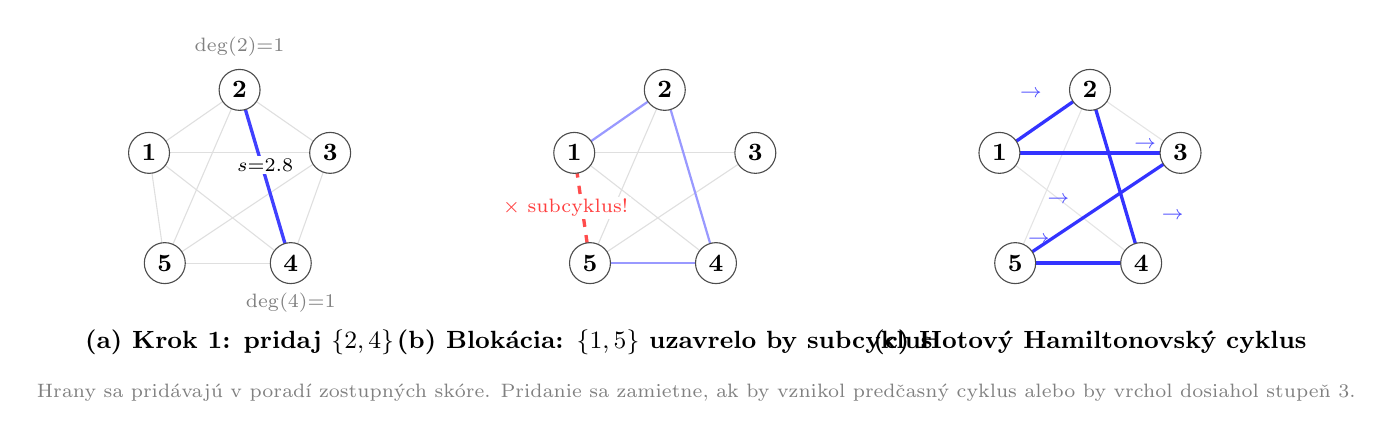
\begin{tikzpicture}[
    font=\small,
    vtx/.style={
        circle, draw=black!70, fill=white,
        minimum size=0.52cm, inner sep=1pt, font=\small\bfseries
    },
    %% Pridaná hrana (aktuálny krok)
    newedge/.style={draw=blue!75, very thick},
    %% Existujúca hrana (z predchádzajúcich krokov)
    oldedge/.style={draw=blue!40, thick},
    %% Zakázaná hrana (subcyklus)
    blocked/.style={draw=red!70, very thick, dashed},
    %% Kompletná trasa
    touredge/.style={draw=blue!80, very thick},
    %% Skóre hrany
    scrlbl/.style={font=\scriptsize, fill=white, inner sep=1pt},
    %% Krížik pre blokovanú hranu
    crosslbl/.style={font=\scriptsize, red!75, fill=white, inner sep=1pt}
]

%% ══════════════════════════════════════════════════════════════════
%% PANEL (a) — Krok 1: pridanie najlepšej hrany
%% ══════════════════════════════════════════════════════════════════
\begin{scope}[xshift=0cm, yshift=0cm]
    %% Vrcholy — 5-uholník
    \coordinate (a1) at (1.15, 2.20);
    \coordinate (a2) at (2.30, 3.00);
    \coordinate (a3) at (3.45, 2.20);
    \coordinate (a4) at (2.95, 0.80);
    \coordinate (a5) at (1.35, 0.80);

    %% Všetky hrany sivé (neskórované)
    \foreach \u/\v in {a1/a2, a1/a3, a1/a4, a1/a5,
                       a2/a3, a2/a4, a2/a5,
                       a3/a4, a3/a5, a4/a5} {
        \draw[draw=gray!25, thin] (\u) -- (\v);
    }

    %% Najlepšia hrana — pridáva sa teraz
    \draw[newedge] (a2) -- (a4)
        node[midway, scrlbl, yshift=4pt] {\(s{=}2.8\)};

    %% Vrcholy
    \foreach \v/\lbl in {a1/1, a2/2, a3/3, a4/4, a5/5} {
        \node[vtx] at (\v) {\lbl};
    }

    %% Stupeň vrcholov
    \node[font=\scriptsize, gray] at (2.30, 3.55)
        {\(\deg(2){=}1\)};
    \node[font=\scriptsize, gray] at (2.95, 0.30)
        {\(\deg(4){=}1\)};

    \node[font=\bfseries\small] at (2.30, -0.20)
        {(a) Krok 1: pridaj \(\{2,4\}\)};
\end{scope}

%% ══════════════════════════════════════════════════════════════════
%% PANEL (b) — Krok N: blokácia subcyklu
%% ══════════════════════════════════════════════════════════════════
\begin{scope}[xshift=5.4cm, yshift=0cm]
    \coordinate (b1) at (1.15, 2.20);
    \coordinate (b2) at (2.30, 3.00);
    \coordinate (b3) at (3.45, 2.20);
    \coordinate (b4) at (2.95, 0.80);
    \coordinate (b5) at (1.35, 0.80);

    %% Ostatné hrany sivé
    \foreach \u/\v in {b1/b3, b1/b4, b2/b5, b3/b5} {
        \draw[draw=gray!25, thin] (\u) -- (\v);
    }

    %% Existujúce hrany v čiastočnom cykle
    \draw[oldedge] (b2) -- (b4);
    \draw[oldedge] (b1) -- (b2);
    \draw[oldedge] (b4) -- (b5);

    %% Blokovaná hrana — uzavrela by subcyklus {1,2,4,5}
    \draw[blocked] (b1) -- (b5)
        node[midway, crosslbl, xshift=-6pt] {\(\times\) subcyklus!};

    %% Vrcholy
    \foreach \v/\lbl in {b1/1, b2/2, b3/3, b4/4, b5/5} {
        \node[vtx] at (\v) {\lbl};
    }

    \node[font=\bfseries\small] at (2.30, -0.20)
        {(b) Blokácia: \(\{1,5\}\) uzavrelo by subcyklus};
\end{scope}

%% ══════════════════════════════════════════════════════════════════
%% PANEL (c) — Finálny Hamiltonovský cyklus
%% ══════════════════════════════════════════════════════════════════
\begin{scope}[xshift=10.8cm, yshift=0cm]
    \coordinate (c1) at (1.15, 2.20);
    \coordinate (c2) at (2.30, 3.00);
    \coordinate (c3) at (3.45, 2.20);
    \coordinate (c4) at (2.95, 0.80);
    \coordinate (c5) at (1.35, 0.80);

    %% Všetky hrany sivé
    \foreach \u/\v in {c1/c3, c1/c4, c2/c5, c3/c5, c2/c3} {
        \draw[draw=gray!20, thin] (\u) -- (\v);
    }

    %% Hotová trasa: 1→2→4→5→3→1  (5 hrán)
    \draw[touredge] (c1) -- (c2);
    \draw[touredge] (c2) -- (c4);
    \draw[touredge] (c4) -- (c5);
    \draw[touredge] (c5) -- (c3);
    \draw[touredge] (c3) -- (c1);

    %% Vrcholy
    \foreach \v/\lbl in {c1/1, c2/2, c3/3, c4/4, c5/5} {
        \node[vtx] at (\v) {\lbl};
    }

    %% Smer trasy — malé šípky
    \node[font=\scriptsize, blue!70] at (1.55, 2.95)  {\(\to\)};
    \node[font=\scriptsize, blue!70] at (3.00, 2.30)  {\(\to\)};
    \node[font=\scriptsize, blue!70] at (3.35, 1.40)  {\(\to\)};
    \node[font=\scriptsize, blue!70] at (1.65, 1.10)  {\(\to\)};
    \node[font=\scriptsize, blue!70] at (1.90, 1.60)  {\(\to\)};

    \node[font=\bfseries\small] at (2.30, -0.20)
        {(c) Hotový Hamiltonovský cyklus};
\end{scope}

%% ══════════════════════════════════════════════════════════════════
%% Spoločný popis pod panelmi
%% ══════════════════════════════════════════════════════════════════
\node[font=\scriptsize, gray, align=center] at (8.1, -0.85)
    {Hrany sa pridávajú v poradí zostupných skóre.
     Pridanie sa zamietne, ak by vznikol predčasný cyklus alebo by vrchol dosiahol stupeň~3.};

\end{tikzpicture}
}
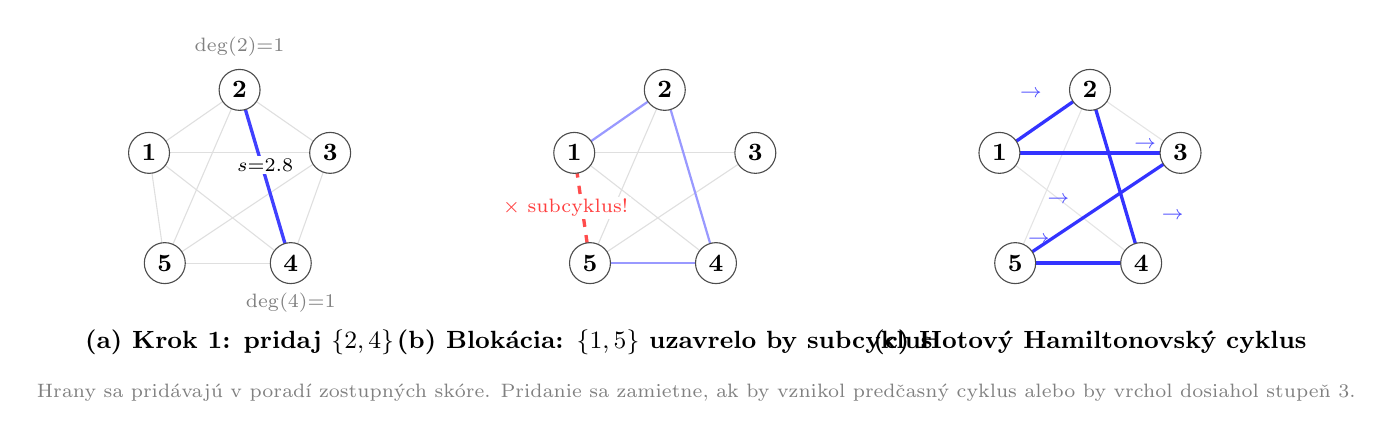
\begin{tikzpicture}[
    font=\small,
    vtx/.style={
        circle, draw=black!70, fill=white,
        minimum size=0.52cm, inner sep=1pt, font=\small\bfseries
    },
    %% Pridaná hrana (aktuálny krok)
    newedge/.style={draw=blue!75, very thick},
    %% Existujúca hrana (z predchádzajúcich krokov)
    oldedge/.style={draw=blue!40, thick},
    %% Zakázaná hrana (subcyklus)
    blocked/.style={draw=red!70, very thick, dashed},
    %% Kompletná trasa
    touredge/.style={draw=blue!80, very thick},
    %% Skóre hrany
    scrlbl/.style={font=\scriptsize, fill=white, inner sep=1pt},
    %% Krížik pre blokovanú hranu
    crosslbl/.style={font=\scriptsize, red!75, fill=white, inner sep=1pt}
]

%% ══════════════════════════════════════════════════════════════════
%% PANEL (a) — Krok 1: pridanie najlepšej hrany
%% ══════════════════════════════════════════════════════════════════
\begin{scope}[xshift=0cm, yshift=0cm]
    %% Vrcholy — 5-uholník
    \coordinate (a1) at (1.15, 2.20);
    \coordinate (a2) at (2.30, 3.00);
    \coordinate (a3) at (3.45, 2.20);
    \coordinate (a4) at (2.95, 0.80);
    \coordinate (a5) at (1.35, 0.80);

    %% Všetky hrany sivé (neskórované)
    \foreach \u/\v in {a1/a2, a1/a3, a1/a4, a1/a5,
                       a2/a3, a2/a4, a2/a5,
                       a3/a4, a3/a5, a4/a5} {
        \draw[draw=gray!25, thin] (\u) -- (\v);
    }

    %% Najlepšia hrana — pridáva sa teraz
    \draw[newedge] (a2) -- (a4)
        node[midway, scrlbl, yshift=4pt] {\(s{=}2.8\)};

    %% Vrcholy
    \foreach \v/\lbl in {a1/1, a2/2, a3/3, a4/4, a5/5} {
        \node[vtx] at (\v) {\lbl};
    }

    %% Stupeň vrcholov
    \node[font=\scriptsize, gray] at (2.30, 3.55)
        {\(\deg(2){=}1\)};
    \node[font=\scriptsize, gray] at (2.95, 0.30)
        {\(\deg(4){=}1\)};

    \node[font=\bfseries\small] at (2.30, -0.20)
        {(a) Krok 1: pridaj \(\{2,4\}\)};
\end{scope}

%% ══════════════════════════════════════════════════════════════════
%% PANEL (b) — Krok N: blokácia subcyklu
%% ══════════════════════════════════════════════════════════════════
\begin{scope}[xshift=5.4cm, yshift=0cm]
    \coordinate (b1) at (1.15, 2.20);
    \coordinate (b2) at (2.30, 3.00);
    \coordinate (b3) at (3.45, 2.20);
    \coordinate (b4) at (2.95, 0.80);
    \coordinate (b5) at (1.35, 0.80);

    %% Ostatné hrany sivé
    \foreach \u/\v in {b1/b3, b1/b4, b2/b5, b3/b5} {
        \draw[draw=gray!25, thin] (\u) -- (\v);
    }

    %% Existujúce hrany v čiastočnom cykle
    \draw[oldedge] (b2) -- (b4);
    \draw[oldedge] (b1) -- (b2);
    \draw[oldedge] (b4) -- (b5);

    %% Blokovaná hrana — uzavrela by subcyklus {1,2,4,5}
    \draw[blocked] (b1) -- (b5)
        node[midway, crosslbl, xshift=-6pt] {\(\times\) subcyklus!};

    %% Vrcholy
    \foreach \v/\lbl in {b1/1, b2/2, b3/3, b4/4, b5/5} {
        \node[vtx] at (\v) {\lbl};
    }

    \node[font=\bfseries\small] at (2.30, -0.20)
        {(b) Blokácia: \(\{1,5\}\) uzavrelo by subcyklus};
\end{scope}

%% ══════════════════════════════════════════════════════════════════
%% PANEL (c) — Finálny Hamiltonovský cyklus
%% ══════════════════════════════════════════════════════════════════
\begin{scope}[xshift=10.8cm, yshift=0cm]
    \coordinate (c1) at (1.15, 2.20);
    \coordinate (c2) at (2.30, 3.00);
    \coordinate (c3) at (3.45, 2.20);
    \coordinate (c4) at (2.95, 0.80);
    \coordinate (c5) at (1.35, 0.80);

    %% Všetky hrany sivé
    \foreach \u/\v in {c1/c3, c1/c4, c2/c5, c3/c5, c2/c3} {
        \draw[draw=gray!20, thin] (\u) -- (\v);
    }

    %% Hotová trasa: 1→2→4→5→3→1  (5 hrán)
    \draw[touredge] (c1) -- (c2);
    \draw[touredge] (c2) -- (c4);
    \draw[touredge] (c4) -- (c5);
    \draw[touredge] (c5) -- (c3);
    \draw[touredge] (c3) -- (c1);

    %% Vrcholy
    \foreach \v/\lbl in {c1/1, c2/2, c3/3, c4/4, c5/5} {
        \node[vtx] at (\v) {\lbl};
    }

    %% Smer trasy — malé šípky
    \node[font=\scriptsize, blue!70] at (1.55, 2.95)  {\(\to\)};
    \node[font=\scriptsize, blue!70] at (3.00, 2.30)  {\(\to\)};
    \node[font=\scriptsize, blue!70] at (3.35, 1.40)  {\(\to\)};
    \node[font=\scriptsize, blue!70] at (1.65, 1.10)  {\(\to\)};
    \node[font=\scriptsize, blue!70] at (1.90, 1.60)  {\(\to\)};

    \node[font=\bfseries\small] at (2.30, -0.20)
        {(c) Hotový Hamiltonovský cyklus};
\end{scope}

%% ══════════════════════════════════════════════════════════════════
%% Spoločný popis pod panelmi
%% ══════════════════════════════════════════════════════════════════
\node[font=\scriptsize, gray, align=center] at (8.1, -0.85)
    {Hrany sa pridávajú v poradí zostupných skóre.
     Pridanie sa zamietne, ak by vznikol predčasný cyklus alebo by vrchol dosiahol stupeň~3.};

\end{tikzpicture}
}
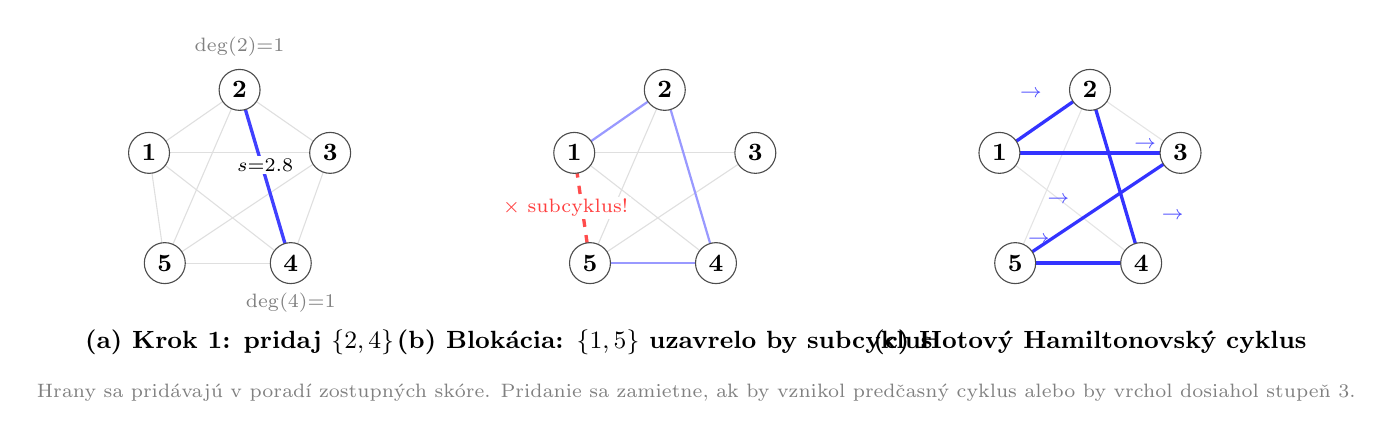
\begin{tikzpicture}[
    font=\small,
    vtx/.style={
        circle, draw=black!70, fill=white,
        minimum size=0.52cm, inner sep=1pt, font=\small\bfseries
    },
    %% Pridaná hrana (aktuálny krok)
    newedge/.style={draw=blue!75, very thick},
    %% Existujúca hrana (z predchádzajúcich krokov)
    oldedge/.style={draw=blue!40, thick},
    %% Zakázaná hrana (subcyklus)
    blocked/.style={draw=red!70, very thick, dashed},
    %% Kompletná trasa
    touredge/.style={draw=blue!80, very thick},
    %% Skóre hrany
    scrlbl/.style={font=\scriptsize, fill=white, inner sep=1pt},
    %% Krížik pre blokovanú hranu
    crosslbl/.style={font=\scriptsize, red!75, fill=white, inner sep=1pt}
]

%% ══════════════════════════════════════════════════════════════════
%% PANEL (a) — Krok 1: pridanie najlepšej hrany
%% ══════════════════════════════════════════════════════════════════
\begin{scope}[xshift=0cm, yshift=0cm]
    %% Vrcholy — 5-uholník
    \coordinate (a1) at (1.15, 2.20);
    \coordinate (a2) at (2.30, 3.00);
    \coordinate (a3) at (3.45, 2.20);
    \coordinate (a4) at (2.95, 0.80);
    \coordinate (a5) at (1.35, 0.80);

    %% Všetky hrany sivé (neskórované)
    \foreach \u/\v in {a1/a2, a1/a3, a1/a4, a1/a5,
                       a2/a3, a2/a4, a2/a5,
                       a3/a4, a3/a5, a4/a5} {
        \draw[draw=gray!25, thin] (\u) -- (\v);
    }

    %% Najlepšia hrana — pridáva sa teraz
    \draw[newedge] (a2) -- (a4)
        node[midway, scrlbl, yshift=4pt] {\(s{=}2.8\)};

    %% Vrcholy
    \foreach \v/\lbl in {a1/1, a2/2, a3/3, a4/4, a5/5} {
        \node[vtx] at (\v) {\lbl};
    }

    %% Stupeň vrcholov
    \node[font=\scriptsize, gray] at (2.30, 3.55)
        {\(\deg(2){=}1\)};
    \node[font=\scriptsize, gray] at (2.95, 0.30)
        {\(\deg(4){=}1\)};

    \node[font=\bfseries\small] at (2.30, -0.20)
        {(a) Krok 1: pridaj \(\{2,4\}\)};
\end{scope}

%% ══════════════════════════════════════════════════════════════════
%% PANEL (b) — Krok N: blokácia subcyklu
%% ══════════════════════════════════════════════════════════════════
\begin{scope}[xshift=5.4cm, yshift=0cm]
    \coordinate (b1) at (1.15, 2.20);
    \coordinate (b2) at (2.30, 3.00);
    \coordinate (b3) at (3.45, 2.20);
    \coordinate (b4) at (2.95, 0.80);
    \coordinate (b5) at (1.35, 0.80);

    %% Ostatné hrany sivé
    \foreach \u/\v in {b1/b3, b1/b4, b2/b5, b3/b5} {
        \draw[draw=gray!25, thin] (\u) -- (\v);
    }

    %% Existujúce hrany v čiastočnom cykle
    \draw[oldedge] (b2) -- (b4);
    \draw[oldedge] (b1) -- (b2);
    \draw[oldedge] (b4) -- (b5);

    %% Blokovaná hrana — uzavrela by subcyklus {1,2,4,5}
    \draw[blocked] (b1) -- (b5)
        node[midway, crosslbl, xshift=-6pt] {\(\times\) subcyklus!};

    %% Vrcholy
    \foreach \v/\lbl in {b1/1, b2/2, b3/3, b4/4, b5/5} {
        \node[vtx] at (\v) {\lbl};
    }

    \node[font=\bfseries\small] at (2.30, -0.20)
        {(b) Blokácia: \(\{1,5\}\) uzavrelo by subcyklus};
\end{scope}

%% ══════════════════════════════════════════════════════════════════
%% PANEL (c) — Finálny Hamiltonovský cyklus
%% ══════════════════════════════════════════════════════════════════
\begin{scope}[xshift=10.8cm, yshift=0cm]
    \coordinate (c1) at (1.15, 2.20);
    \coordinate (c2) at (2.30, 3.00);
    \coordinate (c3) at (3.45, 2.20);
    \coordinate (c4) at (2.95, 0.80);
    \coordinate (c5) at (1.35, 0.80);

    %% Všetky hrany sivé
    \foreach \u/\v in {c1/c3, c1/c4, c2/c5, c3/c5, c2/c3} {
        \draw[draw=gray!20, thin] (\u) -- (\v);
    }

    %% Hotová trasa: 1→2→4→5→3→1  (5 hrán)
    \draw[touredge] (c1) -- (c2);
    \draw[touredge] (c2) -- (c4);
    \draw[touredge] (c4) -- (c5);
    \draw[touredge] (c5) -- (c3);
    \draw[touredge] (c3) -- (c1);

    %% Vrcholy
    \foreach \v/\lbl in {c1/1, c2/2, c3/3, c4/4, c5/5} {
        \node[vtx] at (\v) {\lbl};
    }

    %% Smer trasy — malé šípky
    \node[font=\scriptsize, blue!70] at (1.55, 2.95)  {\(\to\)};
    \node[font=\scriptsize, blue!70] at (3.00, 2.30)  {\(\to\)};
    \node[font=\scriptsize, blue!70] at (3.35, 1.40)  {\(\to\)};
    \node[font=\scriptsize, blue!70] at (1.65, 1.10)  {\(\to\)};
    \node[font=\scriptsize, blue!70] at (1.90, 1.60)  {\(\to\)};

    \node[font=\bfseries\small] at (2.30, -0.20)
        {(c) Hotový Hamiltonovský cyklus};
\end{scope}

%% ══════════════════════════════════════════════════════════════════
%% Spoločný popis pod panelmi
%% ══════════════════════════════════════════════════════════════════
\node[font=\scriptsize, gray, align=center] at (8.1, -0.85)
    {Hrany sa pridávajú v poradí zostupných skóre.
     Pridanie sa zamietne, ak by vznikol predčasný cyklus alebo by vrchol dosiahol stupeň~3.};

\end{tikzpicture}
}
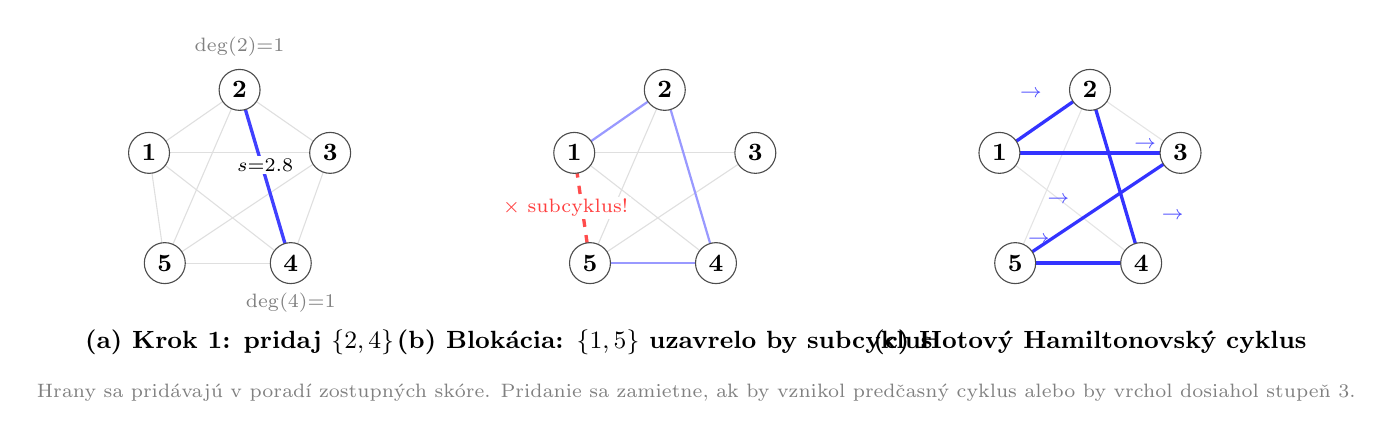
\begin{tikzpicture}[
    font=\small,
    vtx/.style={
        circle, draw=black!70, fill=white,
        minimum size=0.52cm, inner sep=1pt, font=\small\bfseries
    },
    %% Pridaná hrana (aktuálny krok)
    newedge/.style={draw=blue!75, very thick},
    %% Existujúca hrana (z predchádzajúcich krokov)
    oldedge/.style={draw=blue!40, thick},
    %% Zakázaná hrana (subcyklus)
    blocked/.style={draw=red!70, very thick, dashed},
    %% Kompletná trasa
    touredge/.style={draw=blue!80, very thick},
    %% Skóre hrany
    scrlbl/.style={font=\scriptsize, fill=white, inner sep=1pt},
    %% Krížik pre blokovanú hranu
    crosslbl/.style={font=\scriptsize, red!75, fill=white, inner sep=1pt}
]

%% ══════════════════════════════════════════════════════════════════
%% PANEL (a) — Krok 1: pridanie najlepšej hrany
%% ══════════════════════════════════════════════════════════════════
\begin{scope}[xshift=0cm, yshift=0cm]
    %% Vrcholy — 5-uholník
    \coordinate (a1) at (1.15, 2.20);
    \coordinate (a2) at (2.30, 3.00);
    \coordinate (a3) at (3.45, 2.20);
    \coordinate (a4) at (2.95, 0.80);
    \coordinate (a5) at (1.35, 0.80);

    %% Všetky hrany sivé (neskórované)
    \foreach \u/\v in {a1/a2, a1/a3, a1/a4, a1/a5,
                       a2/a3, a2/a4, a2/a5,
                       a3/a4, a3/a5, a4/a5} {
        \draw[draw=gray!25, thin] (\u) -- (\v);
    }

    %% Najlepšia hrana — pridáva sa teraz
    \draw[newedge] (a2) -- (a4)
        node[midway, scrlbl, yshift=4pt] {\(s{=}2.8\)};

    %% Vrcholy
    \foreach \v/\lbl in {a1/1, a2/2, a3/3, a4/4, a5/5} {
        \node[vtx] at (\v) {\lbl};
    }

    %% Stupeň vrcholov
    \node[font=\scriptsize, gray] at (2.30, 3.55)
        {\(\deg(2){=}1\)};
    \node[font=\scriptsize, gray] at (2.95, 0.30)
        {\(\deg(4){=}1\)};

    \node[font=\bfseries\small] at (2.30, -0.20)
        {(a) Krok 1: pridaj \(\{2,4\}\)};
\end{scope}

%% ══════════════════════════════════════════════════════════════════
%% PANEL (b) — Krok N: blokácia subcyklu
%% ══════════════════════════════════════════════════════════════════
\begin{scope}[xshift=5.4cm, yshift=0cm]
    \coordinate (b1) at (1.15, 2.20);
    \coordinate (b2) at (2.30, 3.00);
    \coordinate (b3) at (3.45, 2.20);
    \coordinate (b4) at (2.95, 0.80);
    \coordinate (b5) at (1.35, 0.80);

    %% Ostatné hrany sivé
    \foreach \u/\v in {b1/b3, b1/b4, b2/b5, b3/b5} {
        \draw[draw=gray!25, thin] (\u) -- (\v);
    }

    %% Existujúce hrany v čiastočnom cykle
    \draw[oldedge] (b2) -- (b4);
    \draw[oldedge] (b1) -- (b2);
    \draw[oldedge] (b4) -- (b5);

    %% Blokovaná hrana — uzavrela by subcyklus {1,2,4,5}
    \draw[blocked] (b1) -- (b5)
        node[midway, crosslbl, xshift=-6pt] {\(\times\) subcyklus!};

    %% Vrcholy
    \foreach \v/\lbl in {b1/1, b2/2, b3/3, b4/4, b5/5} {
        \node[vtx] at (\v) {\lbl};
    }

    \node[font=\bfseries\small] at (2.30, -0.20)
        {(b) Blokácia: \(\{1,5\}\) uzavrelo by subcyklus};
\end{scope}

%% ══════════════════════════════════════════════════════════════════
%% PANEL (c) — Finálny Hamiltonovský cyklus
%% ══════════════════════════════════════════════════════════════════
\begin{scope}[xshift=10.8cm, yshift=0cm]
    \coordinate (c1) at (1.15, 2.20);
    \coordinate (c2) at (2.30, 3.00);
    \coordinate (c3) at (3.45, 2.20);
    \coordinate (c4) at (2.95, 0.80);
    \coordinate (c5) at (1.35, 0.80);

    %% Všetky hrany sivé
    \foreach \u/\v in {c1/c3, c1/c4, c2/c5, c3/c5, c2/c3} {
        \draw[draw=gray!20, thin] (\u) -- (\v);
    }

    %% Hotová trasa: 1→2→4→5→3→1  (5 hrán)
    \draw[touredge] (c1) -- (c2);
    \draw[touredge] (c2) -- (c4);
    \draw[touredge] (c4) -- (c5);
    \draw[touredge] (c5) -- (c3);
    \draw[touredge] (c3) -- (c1);

    %% Vrcholy
    \foreach \v/\lbl in {c1/1, c2/2, c3/3, c4/4, c5/5} {
        \node[vtx] at (\v) {\lbl};
    }

    %% Smer trasy — malé šípky
    \node[font=\scriptsize, blue!70] at (1.55, 2.95)  {\(\to\)};
    \node[font=\scriptsize, blue!70] at (3.00, 2.30)  {\(\to\)};
    \node[font=\scriptsize, blue!70] at (3.35, 1.40)  {\(\to\)};
    \node[font=\scriptsize, blue!70] at (1.65, 1.10)  {\(\to\)};
    \node[font=\scriptsize, blue!70] at (1.90, 1.60)  {\(\to\)};

    \node[font=\bfseries\small] at (2.30, -0.20)
        {(c) Hotový Hamiltonovský cyklus};
\end{scope}

%% ══════════════════════════════════════════════════════════════════
%% Spoločný popis pod panelmi
%% ══════════════════════════════════════════════════════════════════
\node[font=\scriptsize, gray, align=center] at (8.1, -0.85)
    {Hrany sa pridávajú v poradí zostupných skóre.
     Pridanie sa zamietne, ak by vznikol predčasný cyklus alebo by vrchol dosiahol stupeň~3.};

\end{tikzpicture}
